\section{Parte I}

\subsection{Q1 - Quatro Scans Diferentes}

Os seguintes comandos serão executados com target o host Metaexploitable 2 que está localizado no IP 172.16.1.130 e a maquina que os executa em 172.16.1.129.

Os comandos executados correspondem a um Host Discovery, a UDP scan, a um TCP Connect Scan e um SYN Scan.Sendo explicados nas próximas secções. 

\subsubsection{Host Discovery}
\hfill\\

O seguinte comando está associado com a descoberta de hosts, também conhecido, como "ping scan".É usado para, de uma forma menos intrusiva e sem fazer scans, detetar os hosts que estão ligados a rede.Em principio, pode ser detetado por IDS,no entanto como pode ser usado também por os administradores de rede seria pouco conveniente bloquear este tipo de trafégo.

\begin{lstlisting}

nmap -sn target

\end{lstlisting}


O resultado do scan ao metasploitable resulta no XML em anexo \ref{sec:nmapsn}.Pelo mesmo podemos ver que o comando detetou que o host está ligado e a responder, devolvendo também o MAC.

Na figura \ref{fig:nmapsn} podemos notar que este tipo de "scan" causa pouco trafégo e passa bastante despercibido para que possa ser detetado visto que faz só um pedido ARP como qualquer outro host na rede.Segundo o manual do nmap devia ter feito um ICMP echo request , um TCP SYN à porta 443 e um TCP ACK à porta 80 ,mas não foi capturado pelo Wireshark.Em todo o caso as mesmas conclusões mantem-se.

\begin{figure}[h!]
	\centering
		
	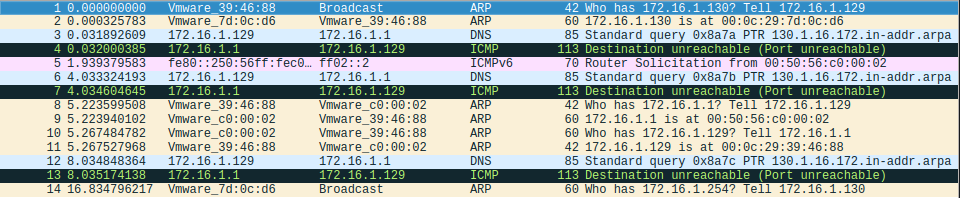
\includegraphics[width=\textwidth,height=3cm,keepaspectratio]{images/nmapsn.png}
		
	\caption{Captura do Wireshark ao nmap -sn}
		
	\label{fig:nmapsn}
\end{figure}

\subsubsection{UDP Scan}
\hfill\\

O seguinte comando é utilizado para fazer scan as portas que respondem a pacotes UDP.Este envia a maioria de pacotes UDP "vazios" excepto o que seja de protocolos especifico para as portas que queramos ou para todas.

As portas podem ser detetadas como quatro estados diferentes open , open filtered, closed, filtered.Caso a "porta" responda,encontra-se no primeiro estado, caso não responda com nada, open filtered.Os outros dois estados depende do ICMP com tipo unreachable error.Caso seja código 3 está closed com outros códigos está filtered.

\begin{lstlisting}

nmap -sU target

\end{lstlisting}

A deteção de portas aberta pode ter vários problemas um deles é que certas portas aberta não respondem a payload vazios e, as Firewall que podem ter filtrado os pacotes também não.Por conseguinte, existe a possiblidade que a porta seja marcada como open filtered.Algumas portas podem ser detetadas com o comando usado para detetar versões já que as respostas que não responderam a pacotes vazios podem responder ao protocolo especifico.Esse comando é usado na secção Q4.

O resultado do scan encontra-se no XML em Anexo \ref{sec:nmapsU}.Existem quatro portas open correspondendo ao serviço domain,rpcbind,netbios-ns,nfs.E três open filtered correspondendo aos serviços dhcpc, tftp, netbios-dgm.

Este filtro o que provoca uma grande quantidade de pacotes serem enviados e recebidos como podemos ver na captura de Wireshark na figura \ref{fig:nmapsULast}.São enviados e recebidos em conjunto 2689 pacotes.

\begin{figure}[h!]
	\centering
		
	
\includegraphics[width=\textwidth,height=3cm,keepaspectratio]{images/nmapLast.png}
		
	\caption{Último pacote gerado por nmap -sU}
		
	\label{fig:nmapsULast}
\end{figure}

Seguidamente, na figura \ref{fig:nmapsUOF} e na figura \ref{fig:nmapsuOpen} podemos ver um exemplo de trafégo para um caso de open filtered e para uma porta open.E, finalmente um caso em que a porta foi determinada como Closed na figura \ref{fig:nmapsUClosed}.

\begin{figure}[h!]
	\centering
		
	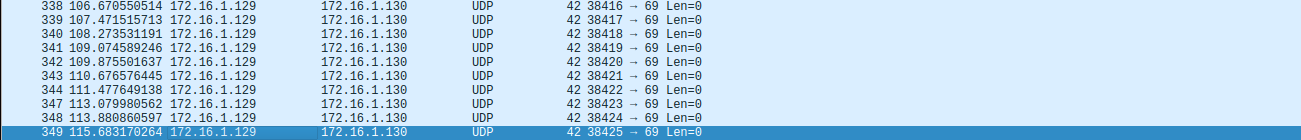
\includegraphics[width=\textwidth,height=3cm,keepaspectratio]{images/nmapSUoF.png}
		
	\caption{Pacotes gerados por um caso de Open Filtered no nmap -sU}
		
	\label{fig:nmapsUOF}
\end{figure}

\begin{figure}[h!]
	\centering
		
	
\includegraphics[width=\textwidth,height=3cm,keepaspectratio]{images/nmapLast.png}
		
	\caption{Pacotes gerados por um caso de Open no nmap -sU}
		
	\label{fig:nmapsuOpen}
\end{figure}

\begin{figure}[h!]
	\centering
		
	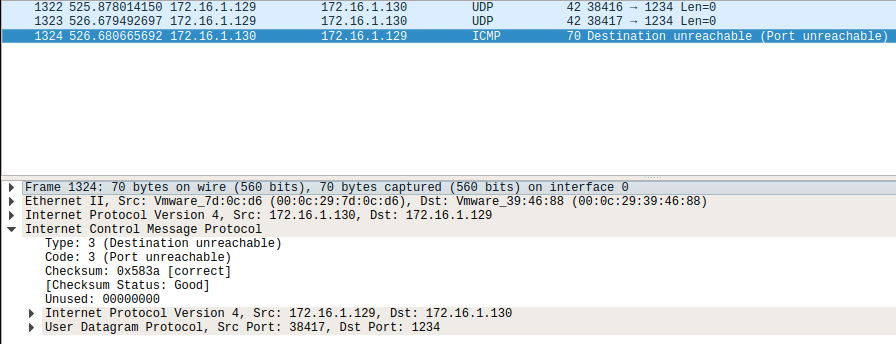
\includegraphics[width=\textwidth,height=3cm,keepaspectratio]{images/nmapsUClosed.png}
		
	\caption{Pacotes gerados por um caso de Closed no nmap -sU}
		
	\label{fig:nmapsUClosed}
\end{figure}

\subsubsection{TCP Connect Scan}
\hfill\\

O seguinte comando é executado quando o SYN scan não é possível.Por exemplo, no caso de redes que sejam IPv6.No entanto, o control sobre este tipo de scan é menor gerando um número maior pacotes para gerar a mesma informação que o SYN scan(Numero de pacotes na figura \ref{fig:nmapsTPacotes}).No entanto, a diferença de pacotes pode não ser muita caso a maioria das portas estejam fechadas.

\begin{lstlisting}

nmap -sT target

\end{lstlisting}

Este modo do nmap realiza o seguinte.Primeiro tenta estabelecer ligação com o host destino através do three-way handshake, seguidamente fecha a conexão usando um pacote RST como pode-se ver na figura \ref{fig:nmapsTConexao}.A título de exemplo um exemplo de conexão falhada na figura \ref{fig:nmapsTNConexao}.

\begin{figure}[h!]
	\centering
		
	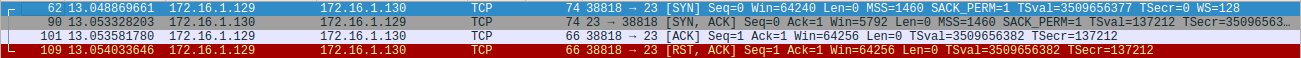
\includegraphics[width=\textwidth,height=3cm,keepaspectratio]{images/nmapsTConexao.png}
		
	\caption{Pacotes gerados por o nmap -sT para una conexão}
		
	\label{fig:nmapsTConexao}
\end{figure}

\begin{figure}[h!]
	\centering
		
	
\includegraphics[width=\textwidth,height=3cm,keepaspectratio]{images/nmapsTNConexao.png}
		
	\caption{Pacotes gerados por o nmap -sT aquando de uma falha na conexão}
		
	\label{fig:nmapsTNConexao}
\end{figure}

O comando gera o XML seguinte que se encontra em Anexo \ref{sec:nmapsT}.
Analisando o XML pode-se ver que foram detetados 23 portas Open para conexões TCP desde o serviço FTP ate o ajp13.O resto das portas foram todas marcadas como Closed.

Um IDS devia detetar este tipo de scan como detetaria o SYN scan que seria mais "leve".No entanto, a maioria não contem este tipo de mecanismo para filtrar os scans.No entanto pode adicionar algum tipo de aviso a um log visto que um host abriu uma conexão e , seguidamente, fechou, sem enviar nenhum tipo de pacotes "úteis".Considerando esse tipo de trafégo como anómalo.

\begin{figure}[h!]
	\centering
		
	
\includegraphics[width=\textwidth,height=3cm,keepaspectratio]{images/nmapsTPacotes.png}
		
	\caption{Número de Pacotes gerado por nmap -sT}
		
	\label{fig:nmapsTPacotes}
\end{figure}

\subsubsection{SYN Scan}
\hfill\\

O SYN Scan é executado com o seguinte comando do nmap.Ao contrário do TCP Connect scan este só envia o packet SYN para "começar" a conexão, no entanto, após receber o SYN ACK do host objetivo lista como Open e deixa o OS enviar um pacote RST para "cortar" o three-way handshake(Figura \ref{fig:nmapsSO}).Caso o próprio servidor retorne um pacote RST então é classificada como Closed(Figura \ref{fig:nmapsSC}).Caso receba nenhuma resposta mesmo de várias tentativas ou receba um ICMP unreachable error então marca como filtered.

\begin{lstlisting}

nmap -sS

\end{lstlisting}

O resultado do XML também encontra-se em Anexo \ref{sec:nmapsS}.Os resultados retirados do mesmo são que existem , como detetado anteriormente, 23 portas Open e 977 portas Closed.Correspondendo aos mesmos serviços encontrados por o TCP Connection Scan.

\begin{figure}[h!]
	\centering
		
	
\includegraphics[width=\textwidth,height=3cm,keepaspectratio]{images/nmapsSO.png}
		
	\caption{Pacotes gerados com nmap -sS resultado em port Open}
		
	\label{fig:nmapsSO}
\end{figure}

\begin{figure}[h!]
	\centering
		
	
\includegraphics[width=\textwidth,height=3cm,keepaspectratio]{images/nmapsSC.png}
		
	\caption{Pacotes gerados com nmap -sS resultado em port Closed}
		
	\label{fig:nmapsSC}
\end{figure}

A seguir podemos ver o numero de pacotes gerados tanto recebidos como enviados na figura \ref{fig:nmapsSPacotes}.
O SYN Scan é menos intrusivo que o TCP Connect Scan já que só executa a primeira parte do three-away handshake e o número de pacotes é menor como referido anteriormente.No entanto necessita privilegios para raw-packets. Apesar destas propriedades ainda pode ser detetado e filtrado por Firewall pessoais e IDS bem configurados.

\begin{figure}[h!]
	\centering
		
	
\includegraphics[width=\textwidth,height=3cm,keepaspectratio]{images/nmapsSPacotes.png}
		
	\caption{Número de Pacotes gerado por nmap -sS}
		
	\label{fig:nmapsSPacotes}
\end{figure}

\subsection{Q2 - Mais Quatro Scans}

Os seguintes nmaps executados verificam que o host scanme (45.33.32.156) está ativo.Os comandos que irão ser executados para cada host , isto é, para o scanme e Metaexploiable 2 serão apresentados, explicados e analisados nas seções seguintes.Estes comandos são especificamente um ACK scan, TCP FIN scan, TCP NULL scan e um TCP Xmas scan.

\subsubsection{ACK Scan}
\hfill\\

O comando seguinte executa um ACK scan para a maquina objetivo.O scan envia pacotes ACK para o host ,não para determinar se as portas estão Open ou Open Filtered, mas ,sim, para determinar se a porta está Filtered ou Unfiltered,ou seja, para determinar o ruleset da Firewall (conjunto de regras que usa para filtrar) e se esta mantêm o registo das conexões ativas presentes no sistema.Caso assim seja, irá filtrar os ACK visto que o nmap não esta conectado ao serviço/porta á qual está direcionada o scan.

\begin{lstlisting}

nmap -sA target

\end{lstlisting}

O scan intrepreta um pacote RST de resposta como Unfiltered(Figura \ref{fig:nmapsAUnfiltered}), caso não haja resposta como Filtered e um ICMP unreachable erro também como filtered.

\begin{figure}[h!]
	\centering
		
	
\includegraphics[width=\textwidth,height=3cm,keepaspectratio]{images/nmapsAUnfiltered.png}
		
	\caption{Pacotes gerados por uma porta Unfiltered com nmap -sA}
		
	\label{fig:nmapsAUnfiltered}
\end{figure}

Ambos os resultados XML para as duas maquinas encontram-se em Anexo \ref{sec:nmapsAmeta} e Anexo \ref{sec:nmapsAscanme}.Ambos apresentam os mesmos resultados.Para as portas 
analisadas foram detetadas todas como unfiltered.Os pacotes gerados pelo nmap são por volta dos 2000 para as duas maquinas no total(enviados mais recebidos) como pode-se ver nas seguintes figuras.

\begin{figure}[h!]
	\centering
		
	
\includegraphics[width=\textwidth,height=3cm,keepaspectratio]{images/nmapsAPacotesMeta.png}
		
	\caption{Número total de pacotes gerados pelo scan -sA para a Metaexploitable 2}
		
	\label{fig:nmapsAPacotesMeta}
\end{figure}

\begin{figure}[h!]
	\centering
		
	
\includegraphics[width=\textwidth,height=3cm,keepaspectratio]{images/nmapsAPacotesScanme.png}
		
	\caption{Número total de pacotes gerados pelo scan -sA para o Scanme}
		
	\label{fig:nmapsAPacotesScanme}
\end{figure}

\subsubsection{TCP FIN,NULL,Xmas Scan}
\hfill\\

Os três comandos seguintes executam, respetivamente, um TCP FIN scan , TCP NULL Scan e um TCP Xmas Scan. Todos eles exploram uma "vulnerabilidade" presente no RFC do TCP que diz "if the [destination] port state is CLOSED .... an incoming segment not containing a RST causes a RST to be sent in response." também não responde com RST caso seja um SYN ou um ACK.O objetivo dos comandos descobrir quais as portas que estão Closed e quais estão Open.

O TCP FIN scan marca a flag que representa que o pacote é um FIN.

\begin{lstlisting}

nmap -sF

\end{lstlisting}

O TCP NULL scan deixa as flags do header a 0 , isto é, deixa o pacote sem tipo.

\begin{lstlisting}

nmap -sN

\end{lstlisting}

O TCP Xmas scan marca todas as Flags que pode, ou seja, FIN, PSH e URG.

\begin{lstlisting}

nmap -sX

\end{lstlisting}

A intrepretação pode ser Open Filtered caso não haja resposta.Caso seja um pacote RST está Closed.E, caso , seja um ICMP unreachable error então a porta esta Filtered.

Estes tipos de scan pode passar mais desaparcebidos que um ACK scan ou que até um SYN scan atraves de Firewall que não mantenham registo das ligações.No entanto, existem três problemas com este tipo de scan.

Primeiro,os IDS modernos já podem ser configurados para detetar este tipo de scan.Segundo, nem todos os sistemas seguem o RFC do TCP implementando todos os aspetos.E, por último, pode não ser possível distinguir entre uma porta aberta e uma filtrada já que a Firewall pode simplesmente não responder e filtrar o pacote.

Idealmente, complementar-se-ia este scan com um SYN scan ou outro parecido que possa detetar se as portas estão abertas.Desta forma, os consequentes scans irão "correr" menos portas passando mais desapercibidos.

Analisando os resultados dos nmap's executados direcionados ao Metaexploitable 2.Os três comandos retornam que existem 23 portas Open Filtered, as mesmas descobertas nos scans anteriores.Podemos ver nas figuras \ref{fig:nmapsFmetaC},\ref{fig:nmapsNmetaC},\ref{fig:nmapsXmetaC} exemplos de portas assinaladas como closed e nas figuras \ref{fig:nmapsFmetaOF},\ref{fig:nmapsNmetaOF},\ref{fig:nmapsXmetaOF} de portas sinalizadas como Open Filtered pelos diferentes comandos.Os resultados do nmap estão no Anexo \ref{sec:nmapsFmeta},Anexo \ref{sec:nmapsNmeta} e Anexo \ref{sec:nmapsXmeta}.

\begin{figure}[h!]
	\centering
		
	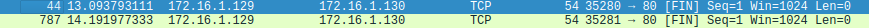
\includegraphics[width=\textwidth,height=3cm,keepaspectratio]{images/nmapsFmetaOF.png}
		
	\caption{Pacotes gerados por o nmap -sF com uma porta Open Filtered para o Metaexploitable 2}
		
	\label{fig:nmapsFmetaOF}
\end{figure}

\begin{figure}[h!]
	\centering
		
	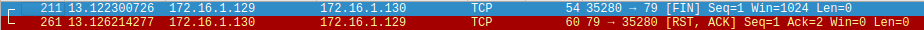
\includegraphics[width=\textwidth,height=3cm,keepaspectratio]{images/nmapsFmetaC.png}
		
	\caption{Pacotes gerados por o nmap -sF com uma porta Closed para o Metaexploitable 2}
		
	\label{fig:nmapsFmetaC}
\end{figure}


\begin{figure}[h!]
	\centering
		
	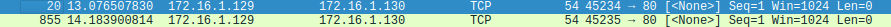
\includegraphics[width=\textwidth,height=3cm,keepaspectratio]{images/nmapsNmetaOF.png}
		
	\caption{Pacotes gerados por o nmap -sN com uma porta Open Filtered para o Metaexploitable 2}
		
	\label{fig:nmapsNmetaOF}
\end{figure}

\begin{figure}[h!]
	\centering
		
	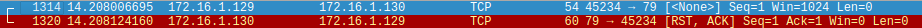
\includegraphics[width=\textwidth,height=3cm,keepaspectratio]{images/nmapsNmetaC.png}
		
	\caption{Pacotes gerados por o nmap -sN com uma porta Closed para o Metaexploitable 2}
		
	\label{fig:nmapsNmetaC}
\end{figure}


\begin{figure}[h!]
	\centering
		
	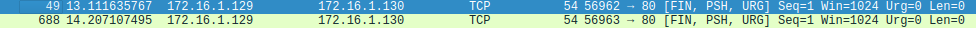
\includegraphics[width=\textwidth,height=3cm,keepaspectratio]{images/nmapsXmetaOF.png}
		
	\caption{Pacotes gerados por o nmap -sX com uma porta Open Filtered para o Metaexploitable 2}
		
	\label{fig:nmapsXmetaOF}
\end{figure}

\begin{figure}[h!]
	\centering
		
	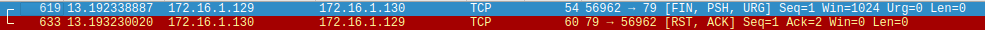
\includegraphics[width=\textwidth,height=3cm,keepaspectratio]{images/nmapsXmetaC.png}
		
	\caption{Pacotes gerados por o nmap -sX com uma porta Closed para o Metaexploitable 2}
		
	\label{fig:nmapsXmetaC}
\end{figure}

Seguidamente, proceder-se-á a analisar os resultados feitos ao host Scanme.Os XML resultantes dos comandos executados estão nos Anexos \ref{sec:nmapsFscanme},\ref{sec:nmapsNscanme},\ref{sec:nmapsXscanme}.Os resultados são todos iguais para as 1000 portas analisadas , isto é, Open Filtered.Combinando com o resultado do ACK scan o mais provável é que as portas estejam todas Open.

Finalmente, do mesmo modo que para a Metaexploitable apresenta-se alguns exemplos de Open Filtered capturados pelo Wireshark aquando do scan feito ao Scanme.Nas figuras \ref{fig:nmapsFscanme},\ref{fig:nmapsNscanme},\ref{fig:nmapsXscanme} são exemplos dos pacotes trocados no caso supra referido pelo TCP FIN scan, TCP NULL scan e o TCP Xmas scan.

O volume de dados encontra-se em volta dos 2000 pacotes também sendo muito parecido entre eles e com ACK scan.

\begin{figure}[h!]
	\centering
		
	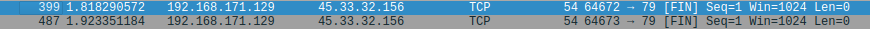
\includegraphics[width=\textwidth,height=3cm,keepaspectratio]{images/nmapsFscanme.png}
		
	\caption{Pacotes gerados por o nmap -sF com uma porta Closed para o Scanme}
		
	\label{fig:nmapsFscanme}
\end{figure}

\begin{figure}[h!]
	\centering
		
	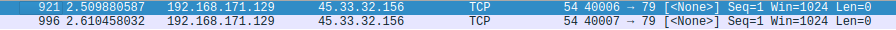
\includegraphics[width=\textwidth,height=3cm,keepaspectratio]{images/nmapsNscanme.png}
		
	\caption{Pacotes gerados por o nmap -sN com uma porta Closed para o Scanme}
		
	\label{fig:nmapsNscanme}
\end{figure}

\begin{figure}[h!]
	\centering
		
	
\includegraphics[width=\textwidth,height=3cm,keepaspectratio]{images/nmapsXscanme.png}
		
	\caption{Pacotes gerados por o nmap -sX com uma porta Closed para o Scanme}
		
	\label{fig:nmapsXscanme}
\end{figure}


